\documentclass{article}
\usepackage{graphicx}
\usepackage[utf8]{inputenc}
\usepackage{fullpage}
\usepackage{titling}
\usepackage{enumitem}
\usepackage{hyperref}
\usepackage[]{algorithm2e}

\parindent0in
\pagestyle{plain}
\thispagestyle{plain}

\newcommand{\assignment}{Práctica 4}
\newcommand{\duedate}{21 de Julio, 2018}

\renewcommand\thesubsection{\arabic{subsection}}

\title{Greedy Problems}
\date{}

\begin{document}

Universidad Católica San Pablo\hfill\\
Algoritmos y Estructura de Datos\hfill\textbf{\assignment}\\
Prof.\ Jorge Poco\hfill\textbf{Entrega:} \duedate\\
Alumno: Moreno Vera Felipe Adrian
\smallskip\hrule\bigskip

{\let\newpage\relax\maketitle}
% \maketitle

\section{Coin Changing}
Consider the problem of making change for $n$ cents using the fewest number of coins. Assume that each coin’s value is an integer.

\begin{enumerate}[label=(\alph*)]
  \item Describe a greedy algorithm to make change consisting of quarters, dimes, nickels, and pennies. Prove that your algorithm yields an optimal solution.
  
  \textbf{Solución:}
  
  Del enunciado y de lo cotidiano, sabemos:
  
  Sea n el número de cambio:\\
  Si $n<5$, usaremos n pennies.\\
  Si $5 \leq n < 10$, usar 1 nickle y n-5 pennies.\\
  Si $10 \leq n < 25$ usar $10\lfloor n/10 \rfloor$ dimes, y luego evaluar los 2 casos anteriores para n - $10\lfloor n/10 \rfloor$.\\
  Si $25 \leq n$, usar $\lfloor n/25 \rfloor$ quarters, y luego evalua los 3 casos anteriores para n - $25 \lfloor n/25 \rfloor$.
  
  Prueba:
  
  Sea $X$ la solución óptima que contiene los tipos de cambio utilizados para brindar la solución.
  
  Hagamos por inducción, que X tenga k tipos de modena, entonces debemos buscar la solución para k+1, como estamos usando algoritmos greedy, se buscará la solución más grande (tipo de moneda) que se aproxime más rápido a k+1. Dado que todos tienen múltiplos de 5, siempre se puede escoger la mejor combinación entre pennies y otros tipos, esto asegura que siempre se hallará la solución óptima.
  
  \item Suppose that the available coins are in the denominations that are powers of $c$, i.e., the denominations are $c^0, c^1, ..., c^k$ for some  integers $c>1$ and $k \geq 1$. Show that the greedy algorithm always yields an optimal solution.
  
  \textbf{Solución:}
  
  Por inducción, tenemos la solución hasta el cambio k-1, es decir tenemos la secuencia $c^0, c^1, ..., c^{k-1}$, entonces cuando tengamos la solución para k, será posible gracias a que son divisibles por c, pero en caso de que no se encuentre una solución óptima, la solución será encontrada haciendo intercambios entre $c_i$ y $c_j$ donde $j>i$.
  
  \item Give a set of coin denominations for which the greedy algorithm does not yield an optimal solution. Your set should include a penny so that there is a solution for every value of $n$.
  
  \textbf{Solución:}
  
  Basta poner números que no cumplan la forma anterior, como: 1, 25, 37.
  
  \item Give an $O(nk)$-time algorithm that makes change for any set of $k$ different coin denominations, assuming that one of the coins is a penny.
  
  \textbf{Solución:}
  
  Ul algoritmo que nos brinde O(nk) para conseguir la combinación de soluciones es Radix Sort con algoritmo estable de Counting Sort en sentido decreciente, debido a que mientras busca las cantidades más cercanas expresadas en monedas ($c_k, c_{k-1}, ..., c_0$ las va tomando por la cantidad de dígitos y las retorna mientras no supere la cantidad a retornar.
  
\end{enumerate}

\section{Maximum-Weight Matching}
Let $G = (V, E)$ be an undirected graph. A subset $F \subseteq E$ of edges is a matching of $G$ if each vertex is the endpoint of at most one edge of $F$.
(Thus each edge of a matching pairs two vertices together, with each vertex paired to at most one other one.) For example, if $G$ is a star on four vertices $u, v, x, y$ (\autoref{fig:ex2}(a)), then the only matchings of $G$ are
the subgraphs with at most one edge (since any two edges overlap in the middle vertex). If $G$ is a three-hop path (\autoref{fig:ex2}(b)), then the first and third edges form a matching; as does the second edge by itself; as does any subset of one of these matchings.

\begin{figure}[h]
  \centering
    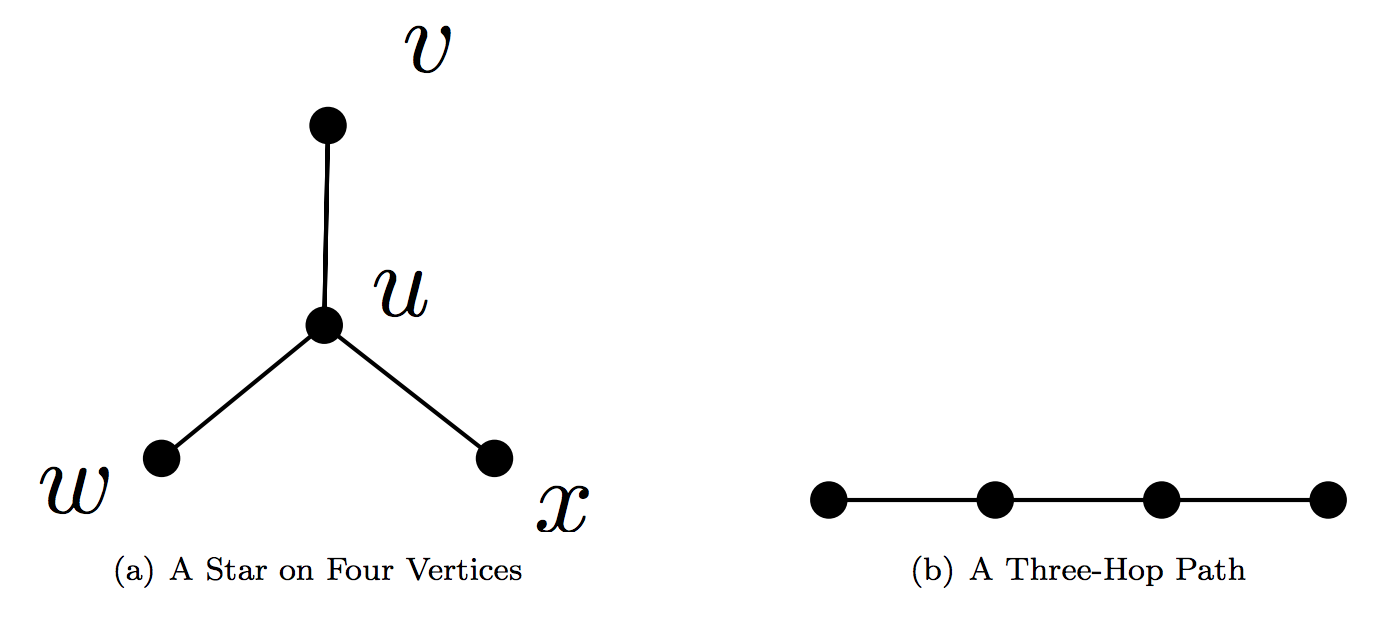
\includegraphics[width=.7\textwidth]{ex12.png}
  \caption{Examples for Problem 2}
  \label{fig:ex2}
\end{figure}

Now suppose that each edge $e$ of $G$ has a nonnegative $weight w_e$. We would like to compute the maximum-weight matching \---\ i.e., the matching with the largest sum of edge weights \---\ or at least a good approximation to it. Here is a natural greedy heuristic, in the spirit of Kruskal's algorithm:

\begin{itemize}
  \item Sort the edges $e_1, ..., e_m$ of $G$ from largest to smallest weight.
  \item $M = \emptyset$
  \item For $i=0$ to $m$:
  \begin{itemize}
    \item if neither endpoint of edge $e_i = (v_i, w_i)$ is already matched \---\ that is, $M$ currently contains no edges incident to either $v_i$ or $w_i$ \---\ then add $e_i$ to $M$.
  \end{itemize}
\end{itemize}

\begin{enumerate}[label=(\alph*)]
  \item Show, by an explicit counterexample, that the algorithm above need not return a maximum-weight matching. For full credit, your counterexample should have the fewest-possible number of edges.
  \item Prove that, for every graph and every set of nonnegative edge weights, the algorithm above returns a matching whose total weight is at least 50\% of that of a maximum-weight matching. 
\end{enumerate}

\section{Gas Station}
You wish to drive from point $A$ to point $B$ along a highway minimizing the time that you are stopped for gas. You are told beforehand the capacity $C$ of you gas tank in liters, your rate $F$ of fuel consumption in liters/kilometer, the rate $r$ in liters/minute at which you can fill your tank at a gas station, and the locations $A=x_1, ..., B = x_n$ of the gas stations along the highway. So if you stop to fill your tank from 2 liters to 8 liters, you would have to stop for $6/r$ minutes. Consider the following two algorithms:

\begin{enumerate}[label=(\alph*)]
  \item Stop at every gas station, and fill the tank with just enough gas to make it to the next gas station.
  \item Stop if and only if you don’t have enough gas to make it to the next gas station, and if you stop, fill the tank up all the way.
\end{enumerate}

For each algorithm either prove or disprove that this algorithm correctly solves the problem. Your proof of correctness must use an exchange argument.\\

\textbf{Solución:}

Para el caso a, si llenamos lo suficientemente para llegar a la otra estación, sea $S=(S_{1,2}, S_{2,3}, ..., S_{n-1,n})$ las respectivas distancias entre los tramos entre cada estación de Gas.

Haciendo una ecuación sencilla tenemos:

F: Tasa de consumo (L/km)\\
C: capacidad del tanque\\
r: tasa de llenado\\
t: Tiempo de llenado (n/r).\\
n: número de litros a llenar.\\

Entonces el número de galones que necesitará para un tramo x = $S_{i,j}$ sería:
$$
  numGalones=S_{i,j} F = (x_j - x_i)F
$$
Y el tiempo de llenado sería:
$$
  tLLenado = numGalones/r = (x_j - x_i)F/r
$$

\textbf{caso A}

El tiempo total de llenado fue: $T(n) = (F/r) \sum_{i=1}^{n-1} (x_{i+1} - x_i)=(F/r) (x_n - x_1) = O(1)$\\
Como hay n paradas, nos tomará O(n).\\

Supongamos por contradicción que esta no es la solución óptima, entonces hay otra solución óptima de las paradas de llenado de tanque, eso implica que ha de detenerse en menor número de estaciones, pero al llenar solo lo necesario para llegar de una estación a otra estación, no llegaría al final del tramo porque le faltaría llenar galones para un tramo.\\

Pero si llenase los galones necesarios para llegar al final en un determinado grifo j, se tendría: $x_{n} - x_j$, pero eso sería igual a $x_{n} - x_{n-1} + x_{n-1} - x_{n-2} + ... + x_{j+1} - x_j$ eso equivaldría a detenerse en todas las estaciones por separado y llenar el tanque. Por lo cual queda demostrado que es la solución óptima del problema.\\

\textbf{caso B}

En este caso, la situación cambia ligeramente, aqui ya no llenamos lo suficiente para llegar de estación a estación, sino nos detenemos exclusivamente si nos quedamos sin gas.

Aqui partiremos de un grifo con el tanque lleno. Entonces desde el punto inicial A partiremos hasta una distancia m (en la cual se nos acabará el gas), cuando se nos este acabando el gas, tendremos que buscar el grifo más cercano para poder recargar.

Como los grifos están continuos unos de otros en el tramo A-B, podemos tomar sus posiciones como ordenadas, entonces durante el trayecto podemos hacer una busqueda binaria.\\
Como hay n grifos, la busqueda no tomará O(logn). Pero como haremos k recargas, el tiempo de busqueda sería O(klogn).\\

Probemos por contradicción que no es la solución óptima:

sea G nuestro conjunto de soluciones de grifos $(G_1, G_2, ..., G_k)$ en k paradas, supongamos que hay otra solución g que contiene k-1 paradas con $(g_1, g_2, ..., g_{k-1})$, entonces empezando desde el primer grifo, tenemos: 

Si $G_i = g_i$, continua a la siguiente parada, hasta la estación k-1, si el auto recarga el tanque lo suficiente como para llegar al final, tenemos $x_{k}-x_{k-1}+x_{k-1}-x_{k-2}$ y esto equivale a haber llegado hasta la estación k.\\
Si $G_i > g_i$, esto no tendría sentido, pues G es la solución óptima, por lo cual se puede tomar que $G_i$ seria igual a $g_i$.
Si $G_i < g_i$, Tal como indica el algoritmo estamos seleccionando la última estación disponible antes de quedarnos sin combustible. si $g_i$ está más lejos que $G_i$ (tomando en cuenta que $g_{k-1} = G_{k-1}$) el auto no llegará y se quedará sin gas.

Entonces hemos probado que si g existe, tiene que ser la misma solución que G. por lo que G es la solución óptima.





%%%%%%%%%%%%%%%%%%%%%%%%%%%%%%%%%%%%%%%%%%%%%%%%%%%%%%%%%%%%%%%%%%%%%%%%%%%%%
%%%%%%%%%%%%%%%%%%%%%%%%%%%%%%%%%%%%%%%%%%%%%%%%%%%%%%%%%%%%%%%%%%%%%%%%%%%%%
%%%%%%%%%%%%%%%%%%%%%%%%%%%%%%%%%%%%%%%%%%%%%%%%%%%%%%%%%%%%%%%%%%%%%%%%%%%%%

\title{Dynamic Programming}
\date{}
\maketitle
\setcounter{section}{0}


\section{Longest Palindrome Subsequence}
A palindrome is a nonempty string over some alphabet that reads the same forward and backward. Examples of palindromes are all strings of length 1, \verb|civic|, \verb|racecar|, and \verb|aibohphobia| (fear of palindromes).

Give an efficient algorithm to find the longest palindrome that is a subsequence of a given input string. For example, given the input \verb|character|, your algorithm should return \verb|carac|. What is the running time of your algorithm?

[Remember to follow the 4 steps explained in the classroom.]

\textbf{Solución:}

Podemos resolver el problema \textit{Longest Palindrome Subsequence} como si fuera el problema \textit{Longest Common Subsequence} usando los pasos de Programación Dinámica.\\

\textbf{Paso 1}

Definimos el problema:

Para una secuencia de caracteres $L = (L_1, L_2, ..., L_n)$, denotamos que una subsecuencia empieza en $L_i$ y termina en $L_j$, tal que $L_ij = (L_i, L_{i+1}, ..., L_j)$.
Sea L nuestra entrada y $L_ij$ la salida dentada como $P=(P_1, P_2, ..., P_m)$, entonces podemos decir:

Sea n la longuitud de L y m la longuitud de P respectivamente

\begin{itemize}

\item Si n=1  entonces m=1 y P=L
\item Si n=2 y $L_1 = L_2$, entonces P=L
\item Si n=2 y $L_1 \neq L_2$, entonces m=1 y P =$L_1$ o P=$L_2$
\item Si $n>2$ y $L_1 = L_n$, entonces $m>2$ y $P_1$ = $P_m$ = $L_1$ = $L_n$ y $P_{2, m-1}$ es un LPS de $L_{2,n-1}$
\item Si $n>2$ y $L_1 \neq L_n$, entonces $P_1 \neq L_1$ indica que $P_{1, m}$ es un LPS de $L_{2,n}$
\item Si $n>2$ y $L_1 \neq L_n$, entonces $P_m \neq L_n$ indica que $P_{1, m}$ es un LPS de $L_{1,n-1}$

\end{itemize}

\textbf{Paso 2}

Luego de definir el problema, podemos dar una solución recursiva asi como a LCS, sea p[i,j] la longuitud de la subsecuencia más larga, tenemos:

\begin{center}
$$
p[i,j] =
   \left \{
      \begin{array}{lclcl}
          1             &, Si & i=j\\
          2             &, Si & j=i+1 &y&  x_i = x_j\\
          1             &, Si & j=i+1 &y & x_i \neq x_j\\
          p[i+1,j-1] + 2&, Si & j>i+1 &y&  x_i = x_j\\
 max(p[i,j-1], p[i+1,j])&, Si & j>i+1 &y & x_i \neq x_j\\
      \end{array}
   \right .
$$
\end{center}

\textbf{Paso 3}

Calculando la longuitud del LPS:

LPS toma una secuencia L como dato de entrada, el algoritmo procesa p[i,j] donde $1 \leq i \leq n$ y p[i,i+1] donde $1 \leq i \leq n-1$ como caso base.

Comienza a llenar los espacios desde p[i,] con $j>i+1$. El algoritmo rellena la tabla p fila por fila, comenzando por la fila n-2 y avanzando hacia la fila 1. (Las filas n-1 y n ya están llenas como parte de los casos base). Dentro de cada fila, el algoritmo llena las entradas de de izquierda a derecha. El algoritmo también mantiene la tabla b[1...n, 1...n] para ayudar a construir la solución optima. 

Algoritmo:

Denotamos los movimientos izquierda, abajo y diagonal izquierda abajo como -1, 0, -2

 \begin{algorithm}[H]
   \caption{LONGEST-PALINDROME}
   LONGEST-PALINDROME; X\\
   n = X.length\\
   Inicializamos b[1..n, 1..n] y p[0..n, 0..n] como nuevas tablas\\
   \For {i = 1 to n-1}{
     p[i, i] = 1\\
     j = i + 1\\
     \If {$x_i == x_j$ }{
       p[i, j] = 2\\
       b[i, j] = -2
     }
     \ElseIf {p[i, j] = 1} {
       b[i, j] = 0
      }
   }
   p[n, n] = 1\\
   \For {i = n-2 to 1}{
     \For {j = i+1 to n}{
       \If {$x_i == x_j$}{
          p[i, j] = p[i + 1, j - 1] + 2\\
          b[i, j] = -2
        }
        \ElseIf {$p[i + 1, j] \geq p[i, j - 1]$}{
           p[i, j] = p[i + 1, j]\\
           b[i, j] = -1
         }
         \ElseIf {p[i, j] = p[i, j - 1]} {
            b[i, j] = izquierda
         }
     }
   }
   \Return  p y b
  \end{algorithm} 
  
  Como se puede notar, el algoritmo toma $\Theta (n^2)$.

\textbf{Paso 4}

Construimos el palindromo. Con el algoritmo anterior, podemos generar el LPS basado en la ruta almacenada en la tabla b, la cual contiene los cambios realizados y evaluados. El algoritmo GENERAR-LPS nos retorna el LPS de la secuencia X

\begin{algorithm}[H]
   \caption{GENERATE-LPS}
   GENERATE-LPS; b, X, i, j, S\\
   \If {$i > j$}{
     return S
   }
   \ElseIf{ i == j }{
     return S || xi
   }
   \ElseIf {b[i, j] == -2}{
     return xi || GENERATE-LPS(b, X, i + 1, j - 1, S) || xi
    }
    \ElseIf {b[i, j] == 0}{
        return GENERATE-LPS(b, X, i + 1, j, S)
    }
    \Else {
      return GENERATE-LPS(b, X, i, j - 1, S)
    }
  \end{algorithm} 
  
% =====================================================================%

\section{Binary Search Tree}

This problem studies the problem of constructing a binary search tree on the keys $\{1, 2, 3, ..., n\}$ that minimizes the weighted search time.

More precisely, you are given as input non-negative weights $w_1, w_2, ..., w_n$ for the keys $\{1, 2, ..., n\}$. The feasible solutions are binary search trees |i.e., binary trees that store the keys $\{1, 2, ..., n\}$ in search tree
order. The search time $T(i)$ for the key $i$ in the tree $T$ is the depth of $i$ in $T$, plus one.


\begin{figure}[h]
  \centering
    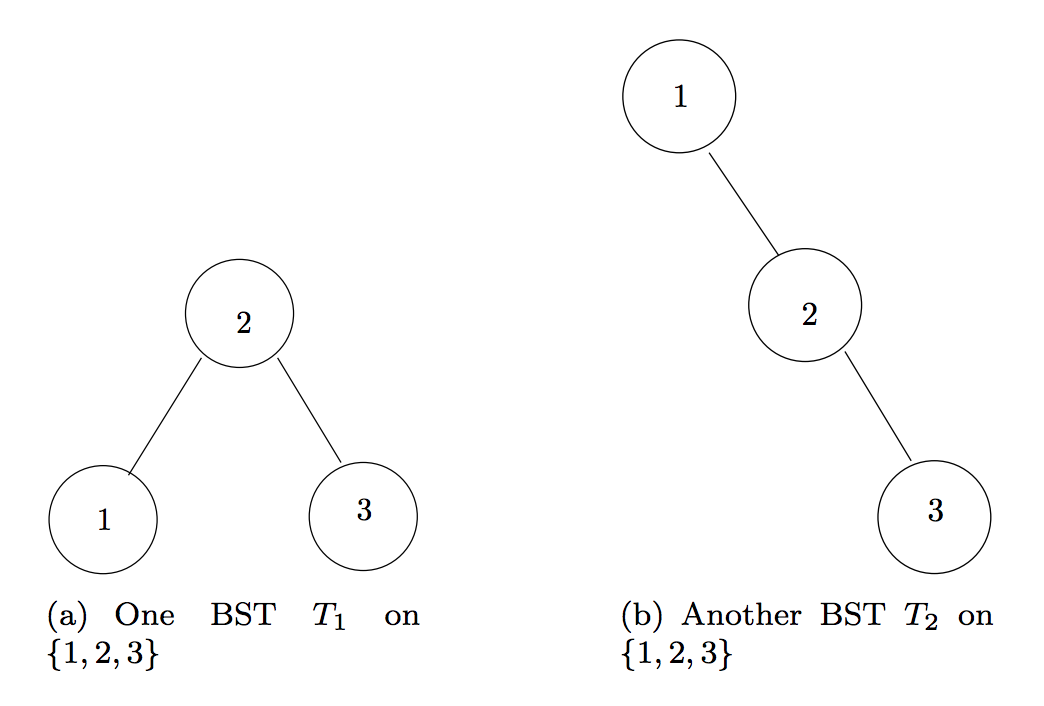
\includegraphics[width=.5\textwidth]{ex22.png}
  \caption{Examples for Problem 2}
  \label{fig:ex2}
\end{figure}

For example, suppose $n=3$. \autoref{fig:ex2} shows two binary search trees on $\{1, 2, 3\}$, $T_1$ and $T_2$. Observe that $T_1(2)=1$ while $T_2(2)=2$.

The weighted search time of a tree $T$ is $\sum_{i=1}^n w_i \cdot T(i)$. For example, if $w1 = w2 = w3 = 2$, then the weighted search time of $T_1$ (namely, $2 \cdot 2 + 2 \cdot 1 + 2 \cdot 2 = 10$) is smaller than that of $T_2$ (namely, 12). On the other hand, if $w_1$ is huge compared to $w_2$ and $w_3$, then the weighted search time of $T_2$ is smaller than that of $T_1$.\\

Give a dynamic programming algorithm that, given non-negative weights $w_1, ..., w_n$, returns the minimum-possible weighted search time of a binary search tree on $\{1, 2, ..., n\}$. (You do not have to construct the tree.) Explain clearly what the subproblems are and what recurrence you use to relate the solutions of
different subproblems to one another. Give a succinct proof that your recurrence is correct. Give a brief analysis of the running time of your algorithm, which should be polynomial in n. 

[Hints: First, what if someone told you which element is the root of an optimal binary search tree? Second, which distinct subproblems do you really need to solve?]


[Remember to follow the 4 steps explained in the classroom.]

\textbf{Solución:}

\textbf{Paso 1}

Definimos el problema:

Para el arbol de pesos $w_i$ para las keys $k_i$ que tienen valor de (1,2,...n), se construye el BST.\\
Planteamos los casos:

El algoritmo encuentra un BST optimo para las diferentes keys $k_i$:

\begin{itemize}
\item Para cada posible raíz $k_r$, para $i \leq r \leq j$.
\item Crea el sub arbol para $k_i, ..., k_{r-1}$.
\item Crea el sub arbol para $k_{r+1}, ..., k_{j}$.
\item Selecciona la raíz que nos da el arbol más óptimo.
\end{itemize}

\textbf{Paso 2}

Luego de definir el problema, podemos dar una solución recursiva, tenemos:\\
Definimos a e(i,j) como el número de comparaciones para el árbol óptimo con keys $k_i, ..., k_j$.

\begin{center}
$$
e(i,j) =
   \left \{
      \begin{array}{lcl}
          0             &, Si & i=j+1\\
 min_{i \leq r \leq j} (e(i,r-1)+e(r+1,j)+w(i,j))&, Si & i \leq j\\
      \end{array}
   \right .
$$
Donde $w(a,b) = \sum_{k=a}^{b} $ es el incremento del costo si $k_a, ..., k_b$ es el subarbol de un nodo.
\end{center}

\textbf{Paso 3}

Calculando la solucón óptima:

Tenemos una serie de valores ordenados definidos como keys $k_1, ..., k_n$\\
Con respectivos pesos $w_1, ..., w_n$\\
El costo de buscar para cada nodo i: costo($k_i$)=profundidad($k_i$)+1\\

Costo esperado: 

CostoTotal = $\sum_{i=1}^{n} costo(k_i) w_i$\\
CostoTotal = $\sum_{i=1}^{n} (profundidad(k_i)+1) w_i$\\
CostoTotal = $\sum_{i=1}^{n} (w_i profundidad(k_i)+w_i)$\\
CostoTotal = $\sum_{i=1}^{n} w_i profundidad(k_i) + \sum_{i=1}^{n} w_i$\\
CostoTotal = $\sum_{i=1}^{n} w_i profundidad(k_i) + O(n)$\\

\textbf{Paso 4}

Construimos el algoritmo basado en la ecuación calculada anteriormente, el algoritmo BST-DP construirá el arbol más óptimo.

\begin{algorithm}[H]
   \caption{BST-DP}
   BST-DP;\\
   \For{size = 1 To n}{
     \For{i=1 To n-size-1}{
        j = i + size -1\\
        e(i,j) = $k_i$\\
        \For{r=i To j}{
           // loop de todas raíz desde $k_i$ hasta $k_j$\\
           t=e(i,j-1)+e(r+1,j) w(i,j)\\
           \If{$t<e(i,j)$}{
             e(i,j) = t\\
             root(i,j) = r
           }
        }
     }
   }
  \end{algorithm} 
  
  Como se puede notar, el algoritmo toma $O(n^3)$.


\section{Binary Search Tree}
Recall that in the standard sequence alignment problem, you are given two strings $X$ and $Y$, of length $n$ and $m$, respectively, over a common alphabet $\Sigma$. The input also includes the penalty $\alpha_{gap}$ of inserting a gap and the penalty $\alpha_{ab}$ of (mis)matching each pair of characters $a$, $b$.

It often makes sense that the penalty for a gap of length 10, say, should be strictly smaller than 10 times the penalty of a single gap. (This reflects the possibility that a large chunk of a genome may get added or deleted via a single ``mutation''.)

To model this, consider a generalization of the sequence alignment problem in which, instead of a single gap penalty $\alpha_{gap}$, the input includes parameters $\alpha_0$, $\alpha_1$, and where the penalty of inserting exactly $k \geq 1$ gaps in a row is $\alpha_0 + \alpha_1 k$. ($\alpha_0$ is larger than $\alpha_1$.) For example, the string AGT can be matched with ACCCGCCT with total penalty $(\alpha_0 + \alpha_1 \cdot 3) + (\alpha_0 + \alpha_1 \cdot 2) = 2\alpha_0 + 5\alpha_1$.

Design a dynamic programming algorithm that correctly solves this generalized sequence alignment problem and runs in $O(mn)$ time. Your algorithm should compute the $value$ (i.e., minimum-possible total penalty) of an optimal alignment; you do $not$ need to produce the alignment itself.

In your answer, explain clearly what the subproblems are, the recurrence(s) you use to relate the solutions of different subproblems to one another, and the order in which you solve the subproblems.
You should give a concise outline of a correctness proof for your
recurrence(s), but don't waste too much time doing it (4-5 sentences
maximum). Also include a brief analysis of the running time of your
algorithm.

[Remember to follow the 4 steps explained in the classroom.]

\end{document}